% ===========================================================================
%  Chapter M, pass 2 --- section files
% ===========================================================================

\section{Markov chains}
\label{m:sec:markov}

The objects of this thesis are Markov chains, in discrete and continuous time,
homogeneous and driven, standing alone and coupled to deterministic dynamics.
This section defines the process classes that recur later: discrete-time chains,
through random walks and Galton--Watson processes; continuous-time chains,
through the Poisson, birth--death and birth--death--catastrophe processes;
time-inhomogeneous chains, through the logistic speciation model; and coupled
ODE--CTMC systems, through the rupture-into-a-medium schematic. The methods for
analysing them are the subject of \cref{m:sec:methods,m:sec:moc}.

\subsection{Discrete-time Markov chains}
\label{m:sec:dtmc}

A \emph{discrete-time Markov chain} is a sequence of \rv s
$\{X_n : n=0,1,2,\dots\}$ taking values in a countable state space
$\mathcal S$ whose future depends on its past only through its present: for all
$n$ and all states,
\begin{equation}
\label{m:eq:dtmcmarkov}
\pr{X_{n+1} = j \mid X_0,\dots,X_n} = \pr{X_{n+1}=j\mid X_n} .
\end{equation}
The chain is \emph{time homogeneous} when the right-hand side depends on $i,j$
but not on $n$, in which case the one-step transition probabilities
\begin{equation*}
p_{ij} = \pr{X_{n+1}=j\mid X_n=i}
\end{equation*}
assemble into the transition matrix $P = (p_{ij})$, whose rows sum to one. The
Chapman--Kolmogorov identity
\begin{equation*}
\pr{X_{n+m}=j\mid X_n=i} = \sum_{k\in\mathcal S}\pr{X_n=k\mid X_n=i}\,p_{kj}^{(m)}
\end{equation*}
shows that the $n$-step transition probabilities are the entries of the matrix
power $P^n$. Every model of this thesis with discrete generations is a chain of
this kind, and the two examples that follow --- random walks and branching
processes --- are the two species of it that recur throughout.

\subsubsection{Simple random walks}
\label{m:sec:rw}

Let $\xi_1,\xi_2,\dots$ be independent \rv s with
$\pr{\xi_k=1}=p$ and $\pr{\xi_k=-1}=q=1-p$, and set
\begin{equation}
\label{m:eq:rwdef}
X_n = X_0 + \xi_1+\cdots+\xi_n .
\end{equation}
The sequence $\{X_n\}$ is a Markov chain on $\mathbb Z$ with transitions
$p_{i,i+1}=p$, $p_{i,i-1}=q$: from any state the walk moves one step right with
probability $p$ and one step left with probability $q$. Its $n$-step law is
explicit. If $R$ of the $n$ increments are $+1$, then
$X_n = X_0 + R-(n-R) = X_0+2R-n$, and $R\sim\text{Binomial}(n,p)$; hence
\begin{equation}
\label{m:eq:rwlaw}
\pr{X_n = X_0+2r-n} = \binom{n}{r}p^{r}q^{\,n-r},
\qquad r=0,1,\dots,n .
\end{equation}
The first two moments follow at once:
\begin{equation*}
\ex{X_n} = X_0 + (p-q)n,
\qquad
\var{X_n} = 4pqn .
\end{equation*}
The walk therefore drifts linearly when $p\neq q$ and diffuses, with variance
growing like $n$, when $p=q=\tfrac12$. \Cref{m:fig:rw} shows the exact law at
$n=40$ for three drifts.

\begin{figure}[ht]
\centering

\includegraphics[width=0.86\textwidth]{figures/rw_transition.pdf}
\caption{Exact position law \cref{m:eq:rwlaw} of the simple random walk at
$n=40$, for $p=0.4$, $0.5$ and $0.6$. The distribution is binomial on the
reachable lattice, centred on the drift $(p-q)n$ with variance $4pqn$; dotted
vertical lines mark the three means. The symmetric walk is the borderline case
between the two drift regimes, and its recurrence is the discrete prototype of
the critical behaviour of \cref{m:app:critical}.}
\label{m:fig:rw}
\end{figure}

Two facts about the symmetric walk are used as standing intuition, and both are
proved by the methods of \cref{m:sec:methdisc,m:sec:methct} rather than by
\cref{m:eq:rwlaw} itself. First, the symmetric walk on $\mathbb Z$ is
\emph{recurrent}: it returns to its starting point, and indeed visits every
state, with probability one, although the expected return time is infinite.
Second, and this is the prototype of every hitting-probability calculation in
this thesis, the probability that the walk reaches a level $b$ before a level
$a<X_0<b$ is determined by a first-step recursion, solved in
\cref{m:sec:methdisc}. The walk is thus the simplest arena in which the two
questions of \cref{m:sec:overview} --- where the process goes, and whether it
gets there at all --- come apart.

\subsubsection{Galton--Watson processes}
\label{m:sec:gw}

The Galton--Watson process is a discrete-time Markov chain on the non-negative
integers in which every member of a population independently either leaves
offspring or does not, at each generational increment. It is the oldest model of
stochastic branching \cite{Harris1963,Athreya1972}, and it is the process on
which most of the rest of this thesis is built. Only the definition and the
one-step structure are set out here; the critical theory is developed in
\cref{m:app:critical}, and the analysis of its quasi-stationary amplitude is the
subject of \ChA.

Suppose each individual produces, independently of every other, a number of
offspring distributed as the \rv{} $L$, with $\pr{L=k}=p_k$ and mean
$\mu=\ex{L}$, and let $Z_n$ be the size of the $n$th generation, started from a
single progenitor, $Z_0=1$. Then
\begin{equation}
\label{m:eq:gwrecursion}
Z_{n+1} = \sum_{i=1}^{Z_n}L_i ,
\end{equation}
the $L_i$ being independent copies of $L$, which makes $\{Z_n\}$ a Markov chain
with transitions from $i$ given by the $i$-fold convolution of the offspring
law. Conditioning on the previous generation gives $\ex{Z_n}=\mu^n$. Writing
$\phi(z)=\ex{z^L}$ for the offspring \pgf, the composition rule of
\cref{m:sec:methdisc} shows that the \pgf{} of $Z_n$ is the $n$-fold composition
of $\phi$ with itself, and in particular the extinction probability
$u_n=\pr{Z_n=0}$ satisfies the iteration
\begin{equation}
\label{m:eq:unIter}
u_{n+1} = \phi(u_n),\qquad u_0=0 ,
\end{equation}
which is the object that \cref{m:sec:methdisc} takes up.

\begin{figure}[ht]
\centering
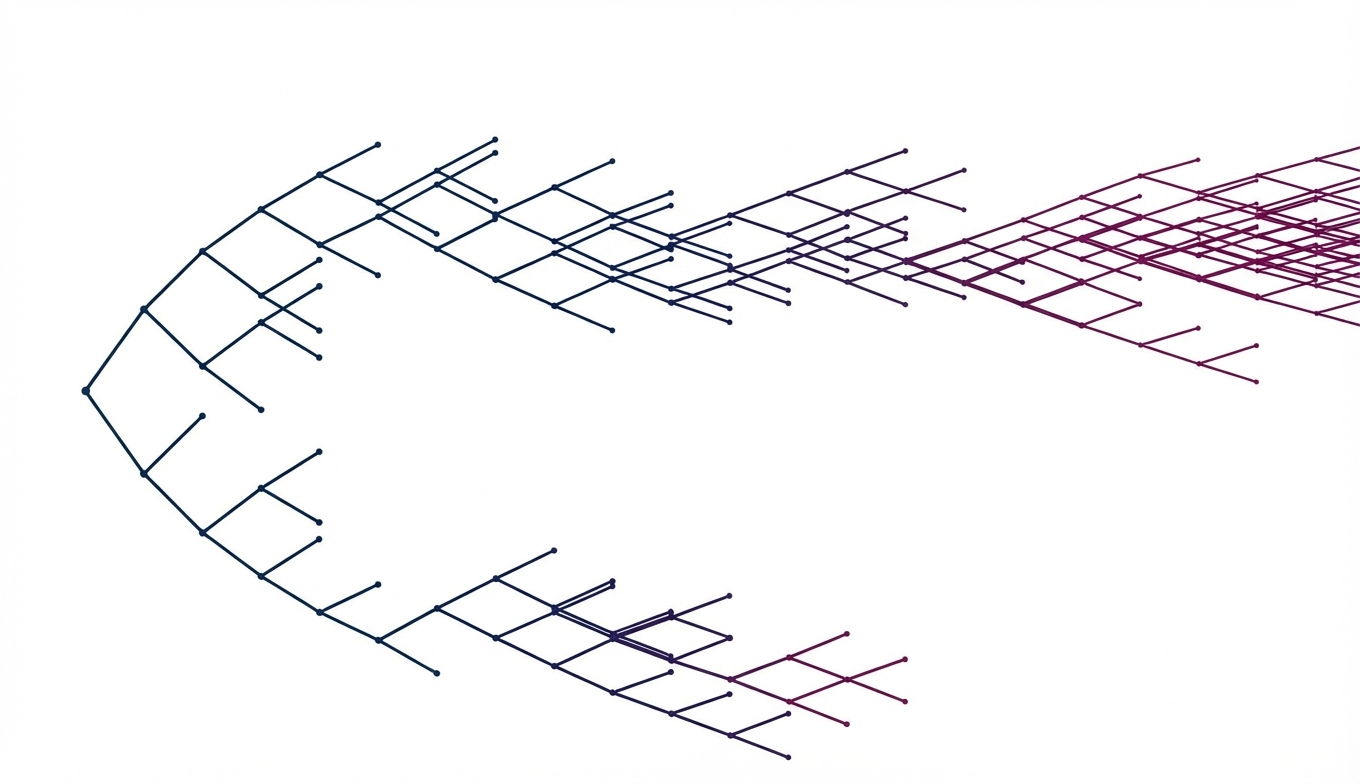
\includegraphics[width=0.78\textwidth]{figures/simpleGWvis.png}\\[6pt]
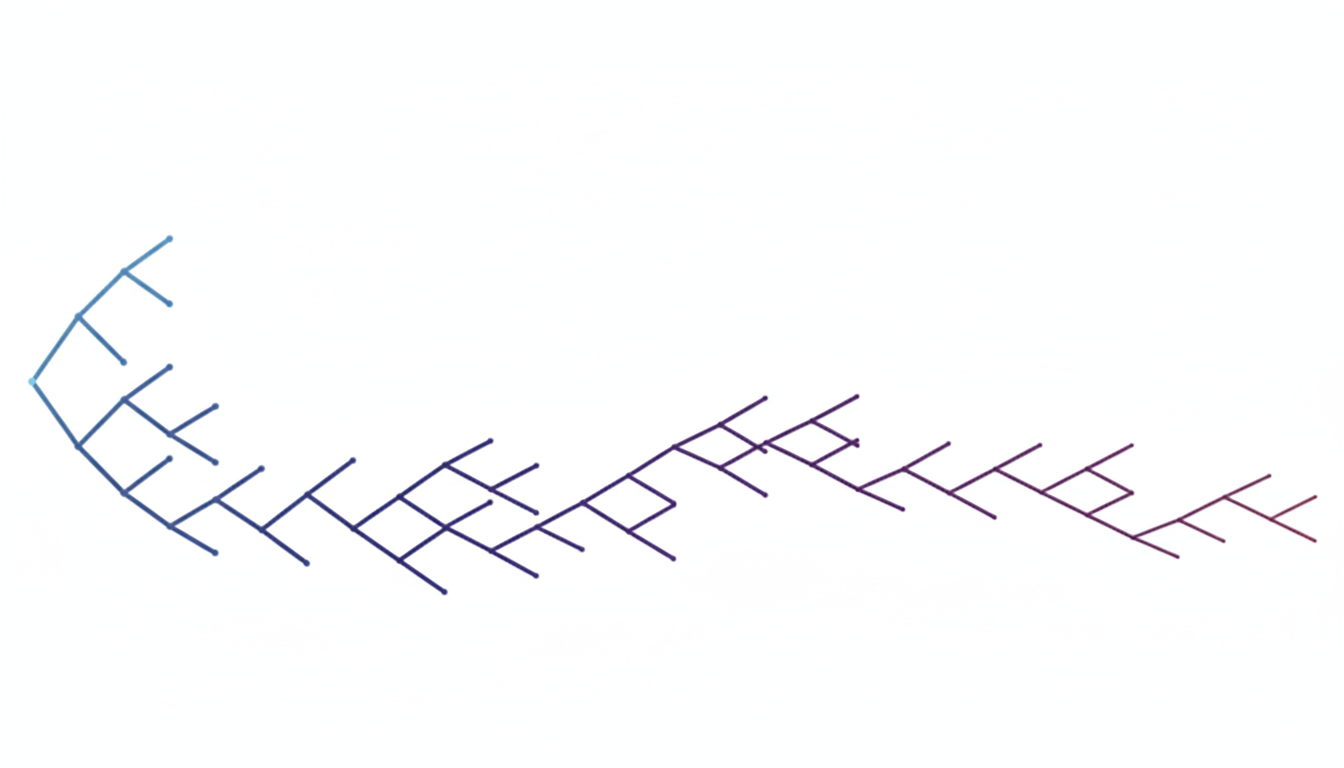
\includegraphics[width=0.78\textwidth]{figures/subGWvis.png}
\caption{Realisations of the simple Galton--Watson process, drawn as genealogies
with generation increasing to the right. Top: supercritical, $p=0.58$, where the
number of lines grows without bound. Bottom: subcritical, $p=0.47$; the same
construction, but the tree terminates. Colour encodes generation number.}
\label{m:fig:gwvis}
\end{figure}

Throughout this thesis we specialise to the binary, or \emph{simple}, case, in
which an individual either divides into two, with probability $p$, or dies, with
probability $1-p$. Then $\mu=2p$, the offspring \pgf{} is
\begin{equation}
\label{m:eq:pgfbinary}
\phi(z) = pz^2 + (1-p),
\end{equation}
and \cref{m:eq:unIter} becomes $u_{n+1} = pu_n^2+1-p$. In terms of the survival
probability $S_n=1-u_n=\pr{Z_n>0}$ the same iteration reads
\begin{equation}
\label{m:eq:SnIter}
S_{n+1} = 2pS_n - pS_n^2,\qquad S_0=1 .
\end{equation}
The process is \emph{subcritical} when $2p<1$, \emph{critical} when
$p=\tfrac12$ and \emph{supercritical} when $2p>1$; extinction is certain in the
first two cases and occurs with probability strictly less than one in the third
(\cref{m:app:critical}). \Cref{m:fig:gwvis} shows realisations either side of the
critical point.

\FloatBarrier
